\chapter{DEM Study on the Evolution of Effective Thermal Conductivity of a Pebble Bed Experiencing Pebble Crushing}\label{sec:dem-studies}
The discrete element method (DEM) is used by many ceramic breeder researchers to model the interaction of individual pebbles in an ensemble in an effort to obtain a more detailed understanding of pebble beds than is possible with experimental measurements of effective properties. For example see Refs.~\cite{An20071393, Lu2000, Zhao2010, Gan2010a, Annabattula2012a, VanLew2014}.

\section{DEM study: effective conductivity with disrupted packing}
\label{sec:dem-studies-effective-conductivity}


Our three-dimensional system consists of mono-dispersed particles of diameter $d$. The particles are constrained by two rigid walls in the $x$-direction at locations of $x = \pm 10d$  and periodic boundary conditions in the $y$-direction located at $y = \pm 7.5d$. Gravity acts in the downward $z$-direction and the particles are bound from below by a rigid wall at $z=0$. The size of the system allows approximately 10~000 particles to fill to a height of approximately $z = 30d$. The volume was chosen to represent the long, tall, narrow channels seen in many solid breeder module designs\cite{ Cho2008, Poitevin2010, Enoeda2003}.
%~~~~~~~~~~~~~~~~~~~~~~~~~~~~~~~~~~~~~~~~~~~~~~~~~~~~~~~~~~~~~~~~~~~~~~



%~~~~~~~~~~~~~~~~~~~~~~~~~~~~~~~~~~~~~~~~~~~~~~~~~~~~~~~~~~~~~~~~~~~~~~
\subsection{Material properties}
For this study, the material was chosen as lithium metatinatate with all properties coming from Ref.~\cite{Gierszewski1998}; they are summarized in Table~\ref{tab:matProps}

\begin {table}[tp] %
\caption{Maximum load and nominal tension.}
\label {tab:matProps} \centering %
\begin {tabular}{ cccccc }
\toprule %
E           &     $\nu$    	&    k         	&    C          &   $\alpha$                \\
(GPa)    	&            	& (W/m-K) 		&  (J/kg-K)  	&   (1/K)                   \\\toprule
126			&      0.24     &  2.5          &  1156       	&   $15\times10^{-6}$		\\\bottomrule
\end{tabular}
\end{table}
%~~~~~~~~~~~~~~~~~~~~~~~~~~~~~~~~~~~~~~~~~~~~~~~~~~~~~~~~~~~~~~~~~~~~~~



%~~~~~~~~~~~~~~~~~~~~~~~~~~~~~~~~~~~~~~~~~~~~~~~~~~~~~~~~~~~~~~~~~~~~~~
\subsection{Methodology}
\label{method}
\begin{figure}[t]
	\centering
	\begin{subfigure}{0.4\textwidth}
		\centering
		\includegraphics[width=\textwidth]{chapters/figures/fill01.png}
	\end{subfigure}
	%\begin{subfigure}[b]{0.15\textwidth}
	%	\centering
	%	\includegraphics[width=\textwidth]{chapters/figures/fill02.png}
	%\end{subfigure}
	\begin{subfigure}{0.4\textwidth}
		\centering
		\includegraphics[width=\textwidth]{chapters/figures/fill03.png}
	\end{subfigure}
	\caption{Demonstrating the pouring process of $N = 10550$ pebbles into the control volume with an early (left) and late (right) snapshot.}
\label{fig:fill01}
\end{figure}

text

\begin{figure}[htbp]
	\centering
	\includegraphics[trim=1cm 8cm 3cm 4cm, width=0.5\textwidth]{chapters/figures/pebbleBedTemperature}
	\caption{Temperature distribution of pebbles in the $10\%$ failed bed. At the end of steady-state heating, a one-dimensional profile is evident in all pebble beds studied here. The pebbles are receiving nuclear heating. Cooling proceeds through the pebbles in contact with the walls in the $x$-direction. [color online]}
\label{fig:pebbleBedTemperature}
\end{figure}

All the test cases begin with a common starting point of a filled, lightly packed volume of 10~550 pebbles. The pebbles are poured into the volume from above and come to rest under the influence of gravity (see Fig.~\ref{fig:fill01}). Initially, to recreate how we may pack solid breeders in reality, we attempted vibration simulations in order to pack the pebbles into a more dense state. However, we found the same packing states (from a void fraction standpoint) could be realized in a more computationally-simple manner by lowering a $z$-plane wall onto the top of the packed bed until it experienced some small force. This pour-press-packing routine was repeated many times and all the beds exhibited the same force on the top wall at roughly the same packing fraction. We took the last case, with a packing fraction (volume of $N$ pebbles per total volume) of $\phi_\text{bl}= 62.9\%$, as our baseline configuration. The packed bed state was saved and used as a starting point for numerous `failed' cases to be described later.

For the baseline case, we assigned an initial temperature of $T_\text{ref}$ to both the pebbles and the $x$ walls, then set a constant nuclear heating source on each pebble. The nuclear energy raised the temperature of the pebbles while the walls remained at $T_\text{ref}$ for cooling. The process ran until a steady state was reached (for example, see Fig.~\ref{fig:pebbleBedTemperature}); the total thermal energy of the bed, $E =\sum_i^N m_iC_i T_i$, was monitored and the simulation completed when the value was constant. At steady state, we analyzed thermomechanical characteristics of the pebble bed such as effective thermal conductivity, average coordination number, temperature profiles in the bed, and inter-particle contact forces.

As mentioned in Sec.~\ref{failureDiscussion}, in this study we model pebble failure without considering the cause of failure. This is done by randomly selecting pebbles from the ensemble, regardless of forces acting upon the pebble, and removing them entirely. When a pebble is removed, the neighboring pebbles react due to the imbalance of forces and the bed settles into a new configuration. We differentiated the failed beds by their percentage of failed pebbles: $\eta = $ number of failed pebbles per original ensemble size. After failing we again applied our heating routine.
%~~~~~~~~~~~~~~~~~~~~~~~~~~~~~~~~~~~~~~~~~~~~~~~~~~~~~~~~~~~~~~~~~~~~~~





%~~~~~~~~~~~~~~~~~~~~~~~~~~~~~~~~~~~~~~~~~~~~~~~~~~~~~~~~~~~~~~~~~~~~~~
\subsection{Pebble Bed Heat Transfer: Test Case}
In our pebble bed test case, we establish heat transfer that is essentially one-dimensional in the $x$-direction. The pebble bed has very little variation of forces and temperatures in the $y$-direction due to the periodic boundary condition at the edges of the domain. Gravity effects are minor in the overall heat transfer and induce only a slight $z$-dependency  to the results. With the one-dimensional assumption, we step back into a continuum mechanics formulation to aid us in finding an effective thermal conductivity of our numeric pebble bed. 

A steady state for a material with constant temperature boundary conditions ($T(\pm 10d) = T_s$) and nuclear heating has the following heat equation

\begin{equation}\label{eq:continuum-heateqn}
	0 = \frac{\mathrm{d}^2T}{\mathrm{d}x^2} + \frac{q'''}{k_\text{eff}}
\end{equation}

In this continuum mechanics formulation, we are assuming that the nuclear source, $q'''$ term is applied evenly over the entire volume. In our DEM formulation, our source term applies to a single pebble. To find the effective thermal conductivity of our pebble bed, we must reconcile this discrepency. This is accomplished  with the exchange of

\begin{equation}
	q''' = \frac{Q_\text{tot}}{V_\text{tot}} = \frac{Q_sN}{300Hd^2}
\end{equation}

where $H$ is the average height of the top layer of pebbles. We apply symmetry about the centerline and impose our boundary conditions to solve the differential equation. If we take the temperature of the midplane as $T(0) = T_0$, we back-out an effective thermal conductivity (ETC) as

\begin{equation}\label{eq:etc}
	k_\text{eff} = \frac{Q_sN}{6H(T_0-T_s)}
\end{equation}


We will use this formulation to analyze and compare our test-case pebble beds.



\begin{figure}[htbp]
	\centering
	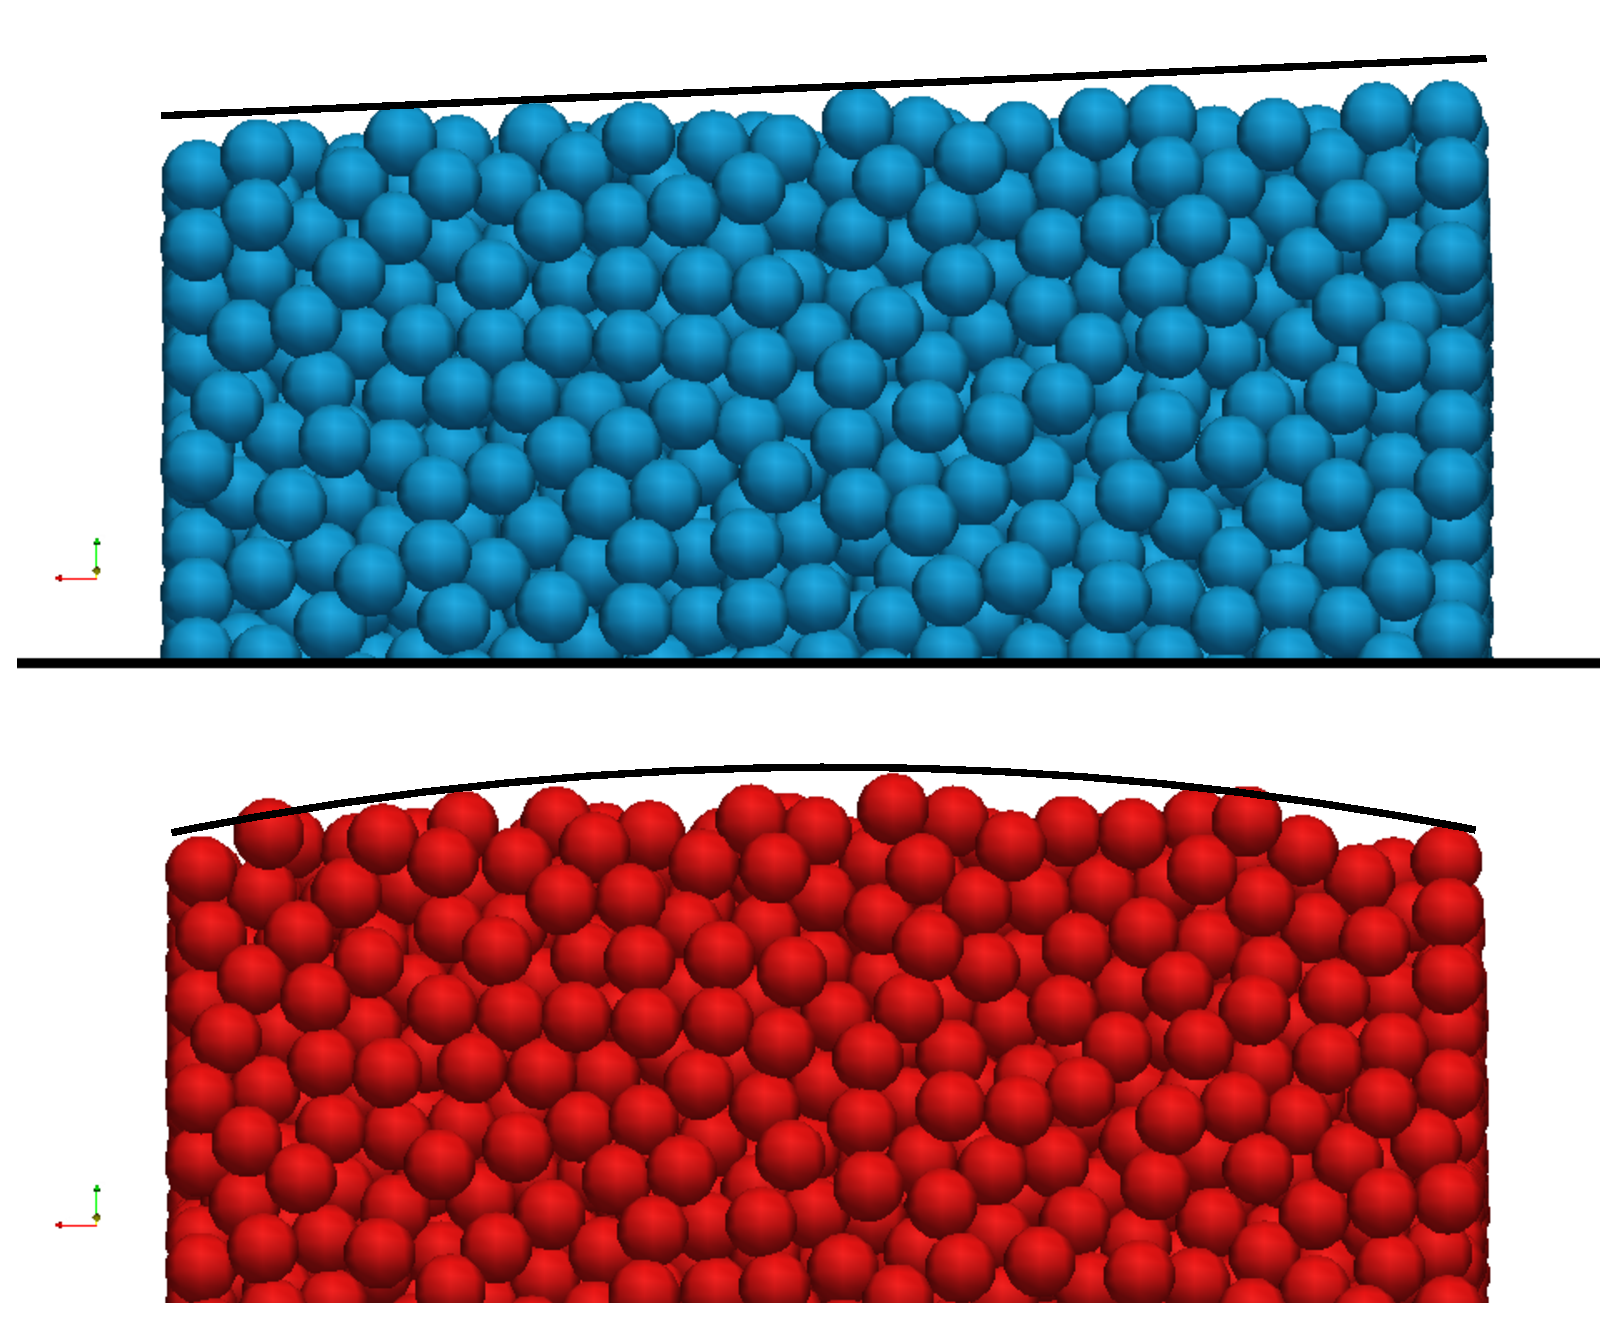
\includegraphics[width=0.5\textwidth]{chapters/figures/settlingStudy}
	\caption{Demonstrating the dynamic resettling from an example study done on location bias to pebble failure. The top image had the pebbles near the left wall biased to fail. The bottom image had a bias for the pebbles near both walls to fail. The lines are drawn as an aid to the eye.}
\label{fig:settlingStudy}
\end{figure}


The aim of this study was both to discover the impact of pebble failure on thermomechanical properties as well as determine the impact as a function of the number of failed pebbles. To satisfy the latter, we created beds with $\eta = 1\%$, $5\%$, $10\%$, and $15\%$ of pebbles failed. 

We first compare steady-state temperature profiles in the test beds against the one-dimensional theory of Eq.\ref{eq:continuum-heateqn}. To find the temperature profile in $x$, we create volumes of width $\Delta x$ that extend through the limits of the $y$- and $z$-directions. We then find the $n$ pebbles residing in the slices and take the mean value of their temperatures, $\langle T\rangle = \sum_{i}^n T_i / n$ of all pebble temperatures that have coordinates inside the slice. Below we will omit the notation $\langle T \rangle$ with the understanding that temperatures are volume-averages. Using the volume slices, we also find the average coordination number, $\langle Z \rangle = \sum_{i}^n Z_i / n$, normalized average contact force, $\langle F^* \rangle=\left[\langle F \rangle/\langle F_{bl} \rangle_\text{max}\right]^{1/3}$, and the normalized average temperature difference between pebbles in the slice, $\langle \Delta T_{ij} \rangle / (T_0 - T_s)_\text{bl}$; parameters which are discussed later.

When analytically solving Eq.~\ref{eq:thermoFirstLaw}, we introduce nondimensional temperature, $\theta_\text{1D} = (T -T_s)/(T_0-T_s)$, and spatial, $x^* = x/L$, variables and the solution becomes purely geometric; $\theta_\text{1D} = 1-x^{*2}$. We plot this theoretical solution against the temperature profiles coming from the steady-state DEM simulation in Fig.~\ref{fig:tempProfile}. We find that all our models had a nearly perfect match to a one-dimensional prediction, validating the calculation of effective thermal conductivity in this study. 

Another concern we had for pebble failure, was the phenomenon of `jamming' during resettling that would possibly leave pebbles isolated from their neighbors (apart from those they are resting upon). Such an isolated pebble would have no strong pathway for heat transfer and heat up much higher than that of its neighbors. Evidence of pebble isolation and `hot-spots' would be apparent in Fig.~\ref{fig:tempProfile} as localized deviations of data points from the quadratic profile. However, no deviations are seen in the data and we conclude that hot-spots will not be a concern in a packed bed.

\begin{figure}[htbp]
	\centering
	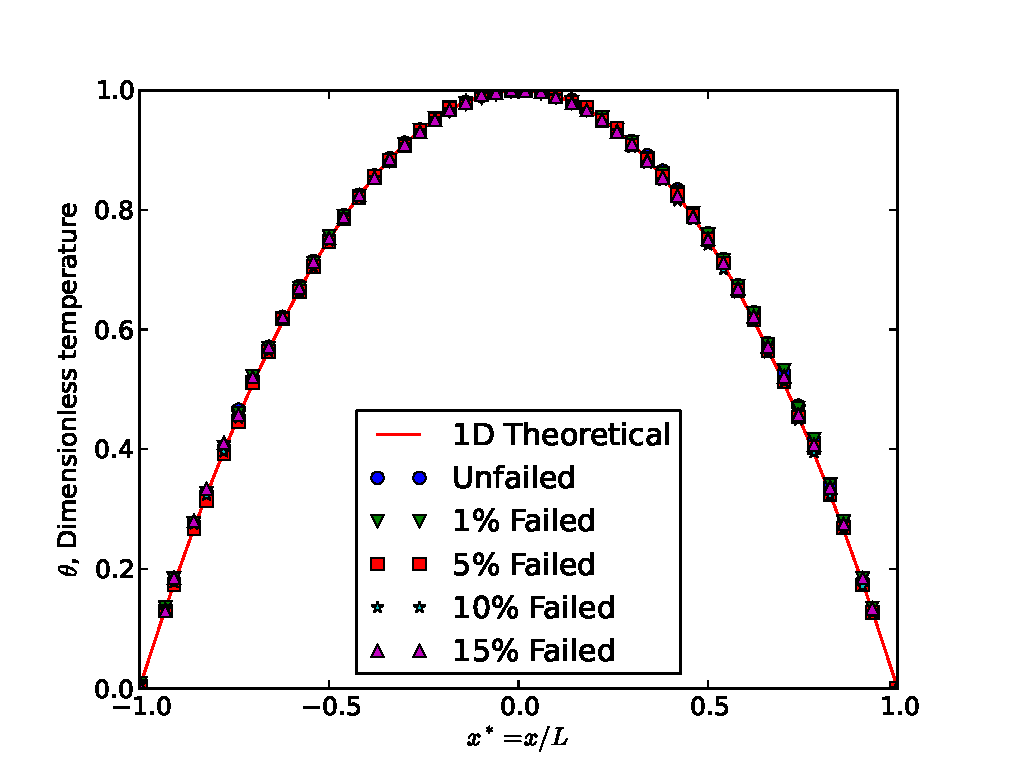
\includegraphics[width=0.65\textwidth]{chapters/figures/tempProfiles}
	\caption{The nondimensional temperature profiles for each test case follow the theoretical shape of a one-dimensional, constant $k$, continuum solution.}
\label{fig:tempProfile}
\end{figure}



\begin{figure}[htbp]
	\centering
	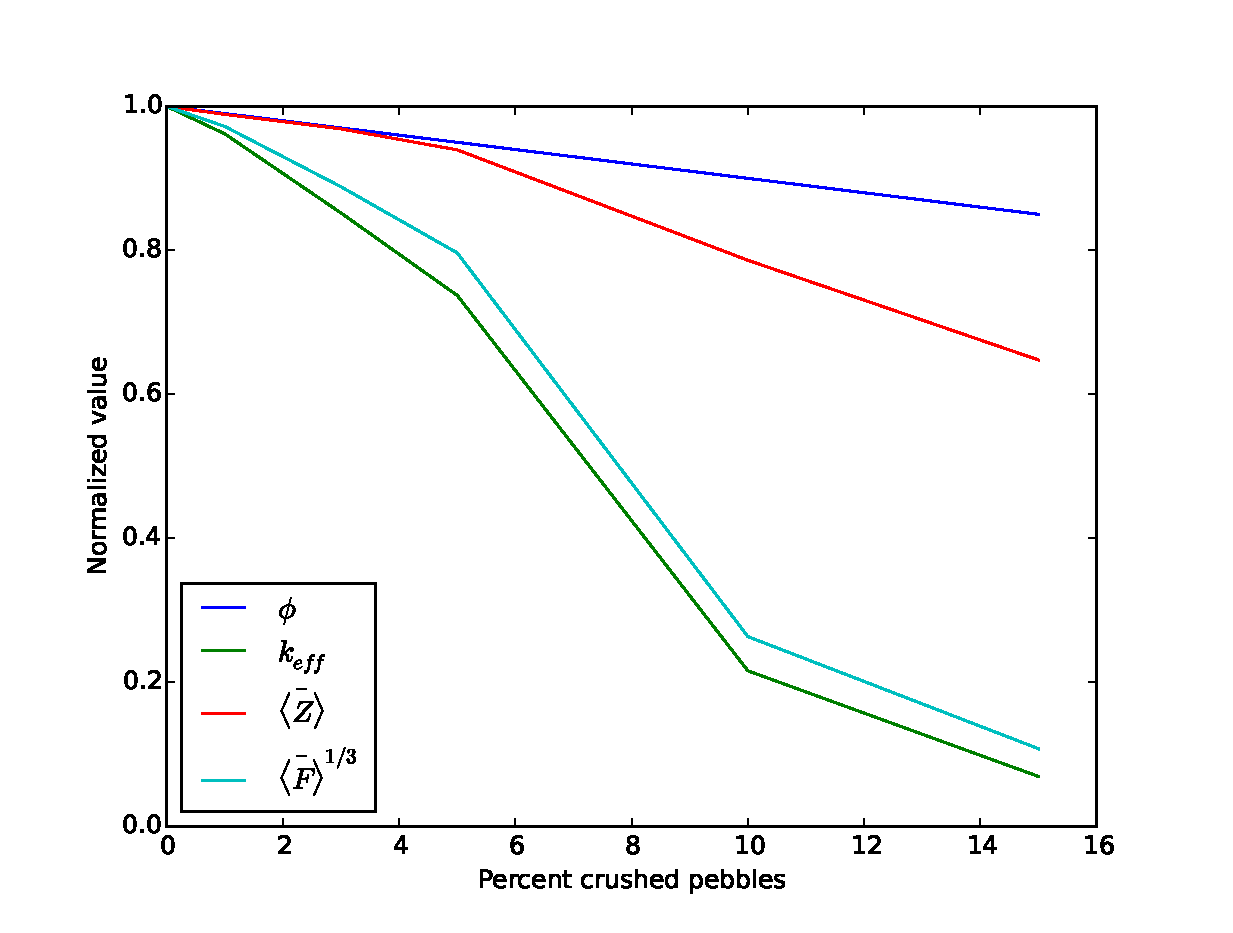
\includegraphics[width=0.65\textwidth]{chapters/figures/kEff_packingFraction}
	\caption{The normalized effective thermal conductivity (solid line) follows an exponential decay relationship with amount of failed pebbles. The normalized packing fraction (dashed line), compared to thermal conductivity, is relatively constant and is more closely fit to a linear reduction.}
\label{fig:packingFraction}
\end{figure}

\begin{figure}[htbp]
	\centering
	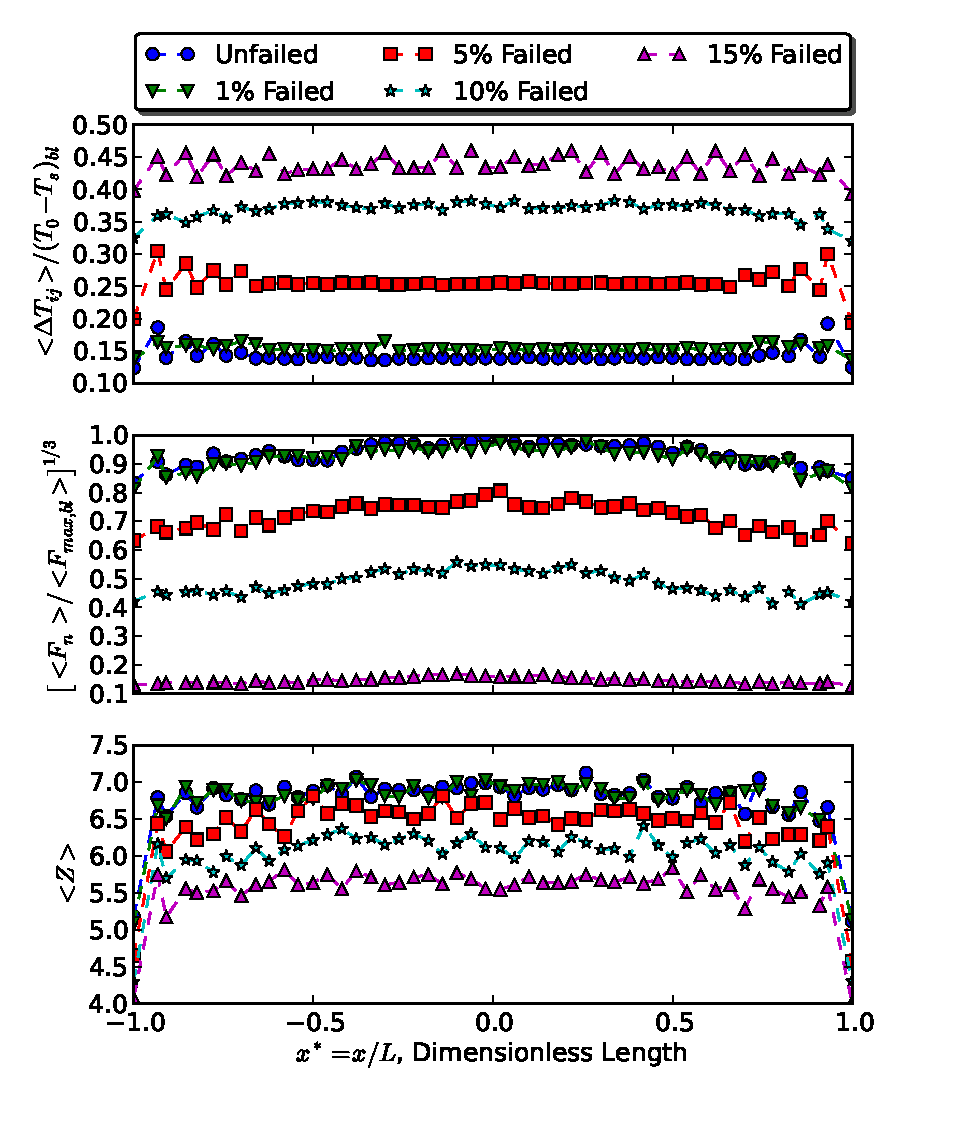
\includegraphics[width=0.75\textwidth]{chapters/figures/z_f_deltaT_subPlots}
	\caption{Average temperature differences between neighboring pebbles (top), contact forces (middle) and coordination numbers (bottom). The profiles of average coordination number and contact forces in the bed decrease in value with increasing pebble failure. Fewer and weaker contacts will reduce the possible paths of heat transfer from a pebble and this results in higher average temperatures between neighbors.}
\label{fig:coordProfiles}
\end{figure}


The effective thermal conductivity is found for all of our pebble beds, via Eq.~\ref{eq:etc}, then normalized against the conductivity of the baseline ensemble ($k_\text{eff}^* = k_\text{failed}/k_\text{bl}$). Figure~\ref{fig:packingFraction} shows the decreasing ETC with pebble failure. When $15\%$ of the pebbles are crushed in a pebble bed, the ETC has fallen all the way to only $k_\text{eff}^*=0.30$. This large reduction is especially important in light of the already poor thermal management of virgin pebble beds that, even in helium environments, have been experimentally measured at only approximately 1~W/m-K (see, { e.g.}, Refs.~\cite{Reimann:2002mi, Piazza2002}). In well-packed pebble beds, the ETC is generally related to the packing fraction. In Fig.~\ref{fig:packingFraction}, this relationship seems weak as the effective conductivity drops much more rapidly than does the packing fraction as the number of broken pebbles in the ensemble increases. To find the cause of decrease in conductivity and to make use of the information provided by DEM tools, we look to other parameters than the packing fraction.

From Eq.~\ref{eq:thermoFirstLaw}, in the steady-state, the energy input by nuclear heating must be balanced by the transport of heat out of a pebble into its neighbors. Inter-particle heat transfer is dictated by the number of neighboring contacts, temperature difference between pebbles, and the thermal conductance, $h_{ij}$ through the contact area. The thermal conductance is, itself, a function of material properties  (which are essentially constant here) and the force at the contact, going as $h_{ij} \propto F_n^{1/3}$. Thus, the net heat out is a function of the three variables as

\begin{equation}
	Q_\text{net} =f( Z, F_n^{1/3}, \Delta T)
\end{equation}



The variables affecting $Q_\text{net}$ are plotted in Fig.~\ref{fig:coordProfiles}. The average coordination number, shown in the bottom plot, decreases from a mid-line value of about 7.0 at the steady-state of the baseline case down to a mid-line value of 5.5 for the 15\% failed bed; a reduction of about 80\%. But this number doesn't compare with the large reduction in ETC which was $k_\text{eff}^*=0.30$. Clearly, there are fewer contacts in the pebble bed after failure but this alone does not account for the reduction in ETC.

Much more dramatic, seen in the center plot, is the reduction in average normal force seen by pebbles after many of the neighbors fail and are removed from the system. From the baseline down to the 15\% failed case, the contact forces are dramatically reduced to about $\langle F^* \rangle=0.1$.This reduction in force is joined by an increase in average neighbor temperatures which are 3 times higher for the bed with most failed pebbles when compared to the baseline. 

The results shown in Fig.~\ref{fig:coordProfiles} demonstrate that the heat transfer through a pebble bed is simultaneously a function of the coordination number and inter-particle contact forces -- which are both reduced as pebbles in the bed fail -- as well as the temperature difference between pebbles at steady state -- which increases as pebbles in the ensemble fail. Interestingly, when a pebble bed has lower overall inter-particle contact forces fewer particles would be expected to break. This would imply that pebble breakage is self-dampening; as pebbles begin to break the ensemble quickly relaxes and avoids future pebble failure. So while we induced failure up to $\eta = 15\%$, such large values may not occur in real beds. 

Another feature of Fig.~\ref{fig:coordProfiles} worth noting is the increase in averaged normal contact forces near the center of the bed relative to the walls. In the assumptions used to develop this simulation, we had noted the lack of localized force concentrations in a bed under an external mechanical load. However, in these results, owing to the nuclear heating temperature profile and thermal expansion of each pebble, there is a bias toward higher forces in the center of the bed. This result highlights the need for a model to predict failure initiation in place of the assumption of random pebble failure. 
%There are dramatic decreases near the walls for two reasons. The first being that contact of a pebble with a wall is not counted in the overall coordination number. The second is the forced ordering that pebbles experience near walls that is absent from the random packing in the bulk. Away from the walls, there is a clear decreasing trend in the coordination number as the pebble failure increases. From Eq.~\ref{eq:thermoFirstLaw}, the heat transfer from a pebble is a function of the number of neighbors with which the pebble is in contact. 


\section{Conclusions}
\label{sec:dem-conclusions}
The results shown in Figs.~\ref{fig:contact-forces-scatter} and~\ref{fig:coord-scatter} demonstrate that the heat transfer through a pebble bed is simultaneously a function of both the coordination number and inter-particle contact forces. The average values of both of these parameters reduced as pebbles in the bed were crushed. Interestingly, when a pebble bed has lower overall inter-particle contact forces such as what we see when pebbles are crushed, we would predict fewer pebbles are likely to break. This result implies that pebble breakage is self-dampening; as pebbles begin to break the ensemble quickly relaxes and avoids future pebble failure. So while in this study we induced failure up to $\eta = 15\%$ without a concern for predicting if such a large amount would break, such large values may not occur in real beds during operation of a fusion reactor. 

The first study of this dissertation established the groundwork of the DEM modeling to be carried out in the other studies. We simulated a pebble bed with a specified fraction of the pebbles crushing during operation; then determining the repercussions of the missing pebbles as they affect the macroscopic property of effective thermal conductivity. We used the assumption of homogeneous, random locations of pebble failure to induce a failure routine without requiring external loads on the bed to actually induce the pebble crushing. After heating to a steady-state, an effective thermal conductivity was calculated for the pebble bed. The results show that large amounts of pebble failure correspond to large decreases in the conductive transport of energy through the pebble bed. The increase was due primarily to a drop in the inter-particle forces which lead to a large increase in temperature differences between neighboring pebbles. 

As the first step in the modeling effort, there were many simplifications that had to be made in this study. We must note here the shortcomings of the assumptions and simplifications of this study before drawing any major conclusions from the results.

First, the `container walls' surrounding the pebble bed in this model are completely rigid and do not react as the swelling pebble bed presses into them while heating. The confined thermal expansion leads to very high contact forces in the pebble bed that may not be realistic. The abnormally high contact forces are most likely to be the source of the abnormally high baseline effective thermal conductivity, $k_0 = 1.03$~W/m-K. In experiments on the effective thermal conductivity of lithium ceramics in vacuum, the beds are often allowed to expand freely while heating (in at least one direction) and in vacuum were measured to be closer to $k_0 = 0.5$ W/m-K [FIND THE REAL VALUES TO PUT HERE!]. We note, however, that this value has been calculated in the absence of interstitial gas so the results apply only to the reduction in energy transferred via inter-particle conduction.

Second, we saw from Fig.\ref{fig:temp-scatters} that the majority of the pebbles in the ensemble have their temperatures close fitting to an average curve but a number of the pebbles had less thermal contact with neighboring particles and consequently had much larger temperatures. This was true even in the baseline case of a tightly packed ($\phi = 64\%$) pebble bed. This phenomena is only possible because the contribution to heat transfer of the interstitial gas was not considered in this model. The flowing helium gas is expected to prevent any runaway temperatures of individual pebbles as it provides another route of energy transfer in the bed. This will be addressed in \cref{sec:cfd-dem-studies}.

Lastly, the pebble crushing did not conserve mass and did not have predictive whatever.